\section{Graphical User Interface for Teleoperation}
	\label{sec:teleoperation_gui}
	
	The Graphical User Interface (GUI) used for the teleoperation of HRP-2Kai was implemented
	in Choreonoid, an integrated robotics GUI environment~\cite{Choreonoid}~\cite{Nakaoka_Choreonoid}.
	A snapshot of this GUI is shown in \figurename~\ref{fig:Choreonoid3}.
	As can be seen, the teleoperation interface features several windows, each one of them
	corresponding to
	%
	\begin{inparaenum}[(1)]
		\item the scene view,
		\item the task sequencer,
		\item the head camera,
		\item the right hand camera,
		\item the left hand camera,
		\item the item view, and
		\item the property view.
	\end{inparaenum}
		
	\begin{figure}[t]
		\centering
		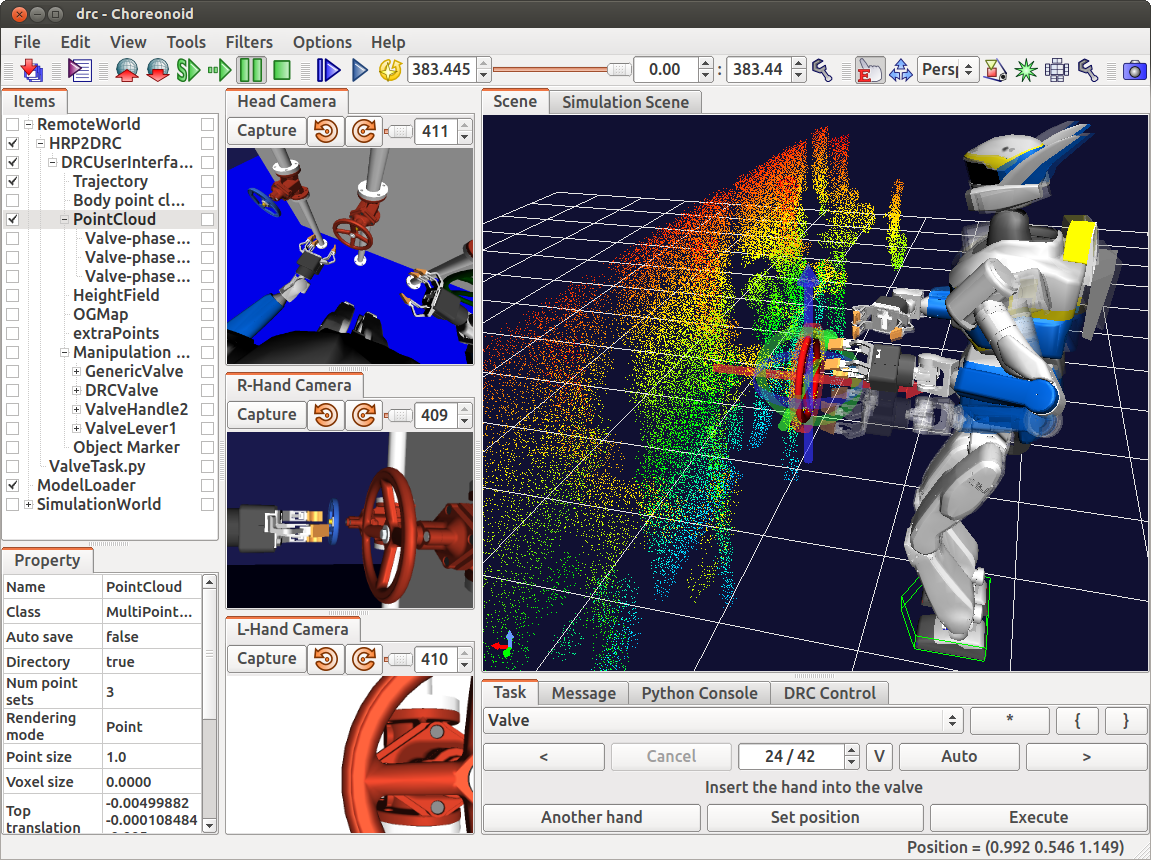
\includegraphics[height = 5.5cm]{img/Choreonoid3}
		\caption{Teleoperation interface in Choreonoid~\cite{Nakaoka_Humanoids}.}
		\label{fig:Choreonoid3}
	\end{figure}
	
	The scene view is used to teleoperate the robot through the direct control of a 3D model
	showing the robot's current configuration, as well as the planned motion represented by
	one (or several) translucent version(s) of the robot, one per each key configuration.
	The \emph{point cloud} of data corresponding to the measured points on the surface of the
	objects in the environment is captured by the 3D scanner and presented also in the scene view.
	From this information it is possible to extract the \emph{height field} of the floor,
	used by the walking control system to achieve a stable gait over uneven terrain~\cite{Morisawa},
	as well as to detect obstacles and objects of interest in the environment in order to perform
	a proper whole-body collision-free posture planning, as required by the manipulation
	task~\cite{Kanoun}.
	
	The object that is the target of the manipulation task can be identified in the point cloud
	by overlapping a simplified 3D model of it, as shown in \figurename~\ref{fig:Choreonoid3}.
	This model, referred as \emph{Manipulation Marker}, provide a reference frame with respect
	to which the manipulation task can be described once it is aligned with the corresponding
	points.
	This alignment can be done manually by using a set of arrows and rings provided by the interface
	to translate and rotate the marker, or automatically with the aid of a built-in function included
	in the Point Cloud Library (PCL), used by Choreonoid.
	
	The manipulation motion is specified by providing the pose (position and orientation)
	of the hands of the robot, and calculated by solving the whole-body inverse kinematics
	problem~\cite{Kanoun}.
	This motion can be either planned in advance or manually changed during the execution of the task
	by using \emph{Hand Markers} (3D models of the hands that can also be translated and rotated).
	
	The \emph{task sequencer} is provided by the interface to execute a manipulation
	task step by step, such that the complex perception and supervision be entrusted to the operator.
	On every step, the robot is commanded to go to a predefined stance and/or to reach a predefined posture,
	both of them relative to a previously identified target.
	Then, the robot autonomously generates the required motion to accomplish the desired configuration,
	avoiding obstacles represented by the point cloud and maintaining its dynamic stability.
	
	Finally, the interface also provides the image captured by every camera, as well as additional information.
	For example, the item window enlists the components required by Choreonoid to implement the teleoperation
	interface, together with their configuration parameters: their properties.
	
	By using this interface we implemented all the manipulation tasks required during the
	DARPA Robotics Challenge:
	%
	\begin{inparaenum}[(1)]
		\item opening a door,
		\item turning a valve,
		\item cutting a wall with a drill, and
		\item a surprise task which consisted in opening a box and pushing a button (rehersal day),
					pulling down a lever (first day of the competition) or
					pulling a plug out of a socket and inserting it into another one (second day of the competition).
	\end{inparaenum}
	%
	Given that the approach to implement each one of them was similar,
	we will only explain two representative ones:
	the door task and the plug task.